\documentclass[../../../main]{subfiles}
\begin{document}
\subsection*{Qudrature Decoder introduction}
The Quadrature Decoder is used to interprete the position of the system's motors using the signals from the two enocders, each  mounted on motor. This subsection will introduce a little theory of a both Qudrature Decoder and encoder and how the Quadrature decoder has been implementated on the FPGA.
\subsection*{Quadrature Encoder}
\label{sub:Theory}

First, in order to understand the implementation of the Quadrature Decoder on the FPGA, a small explanation of how a Quadrature Encoder works is needed. \\
A Quadrature Encoder uses two channels to sense the position of, typically, a rotating disk/shaft or a linear strip. The disk or strip has two paths on it, positioned 90 degresse out of phase of each other, see figure \ref{rotary_encoder} for a rotary encoder and see figure \ref{channels_1} for a strip encoder. Statinoary sensores are typically placed on top of the encoder, so when a track moves in relation to a sensor, it outputs a logic high or low output signal depending on what part of the track is visible to the sensor. An encoder has two output signals, one for each channel, typically called A and B, see figure \ref{channels_2}. This two signals, A and B, is what the decoder uses to determine the position of the encoder.


\begin{figure}[H]
  
\includegraphics[width = \textwidth]{\main/afsnit/system_implementation/Quadraturdecoder/pictures/encoder.png}
  \caption{The figure shows the tracks of a rotary encoder.}
  \label{rotary_encoder}
\end{figure}

\begin{figure}[H]
  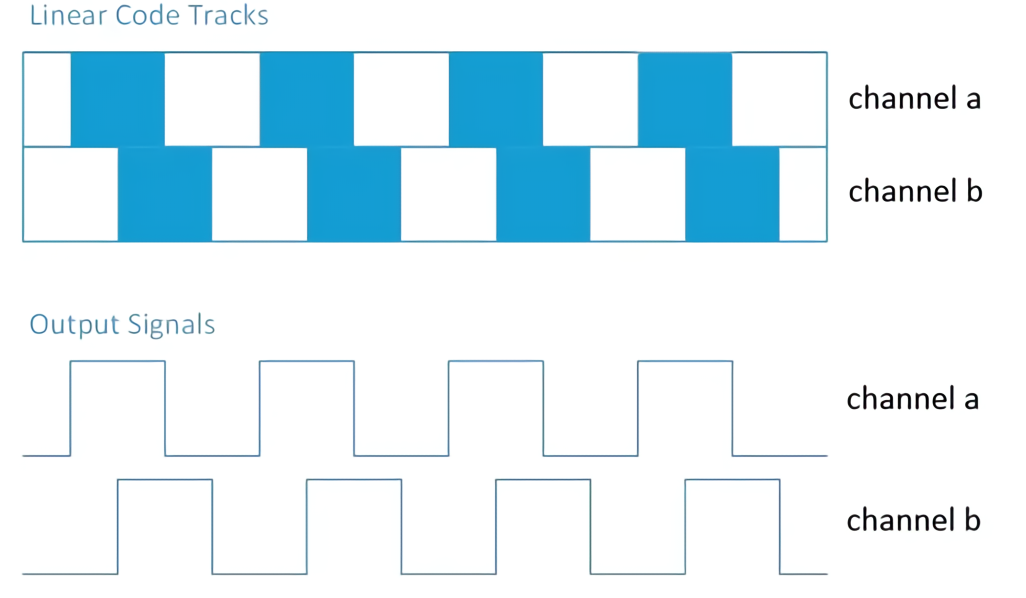
\includegraphics[width = \textwidth]{\main/afsnit/system_implementation/Quadraturdecoder/pictures/channels.png}
  \caption{The figure shows the output of both a rotary and linary encoder}
  \label{channels_1}
\end{figure}

\subsection*{Decoder principle}
The idea with a quadrature Decoder is for it to decode the two output signals the encoder produces and return a position. The idea is to observe the both the encoders outputs. By counting the transitions from high to low and low to high on just one of the outputs, it can be determined how far the encoder has rotated. However, by adding the second output, the direction of the encoder can be computed as well as adding a higher resolution to the position. The encoder used in this project has a resolution of 360, meaning a Quadrature decoder will count 360 for each full rotation. This rotation can of course not be mapped directly to the system itself, since the motors is geared. The motors has to do 3 full rotations before the system itself has made a full roation. Hence the resolution for the system is 1080. This is very useful, since it gives a $\frac{1}{3}$ of a degrees position precision.
\subsection*{implementation}

\begin{tabular}{|c | c | c | c | c | c |c |}
\hline
 A\_prev & A\_new & B\_prev & B\_new & return\_to\_home & Direction & Position \\
 \hline
 0 & 1 & 0 & 0 & 1 & forward & + 1 \\
 1 & 1 & 0 & 1 & 1 & forward & + 1 \\
 1 & 0 & 1 & 1 & 1 & forward & + 1 \\
 0 & 0 & 1 & 0 & 1 & forward & + 1 \\
 0 & 0 & 0 & 1 & 1 & Backwards & - 1 \\
 1 & 0 & 0 & 0 & 1 & Backwards  & - 1 \\
 0 & 1 & 1 & 1 & 1 & Backwards & - 1 \\
 1 & 1 & 1 & 0 & 1 & Backwards & -1 \\
 x & x & x & x & 0 & No change & 0 \\
 \hline
\end{tabular}
\end{document}
